\begin{figure}[htbp!]
	\begin{center}
	\resizebox{\linewidth}{!}{
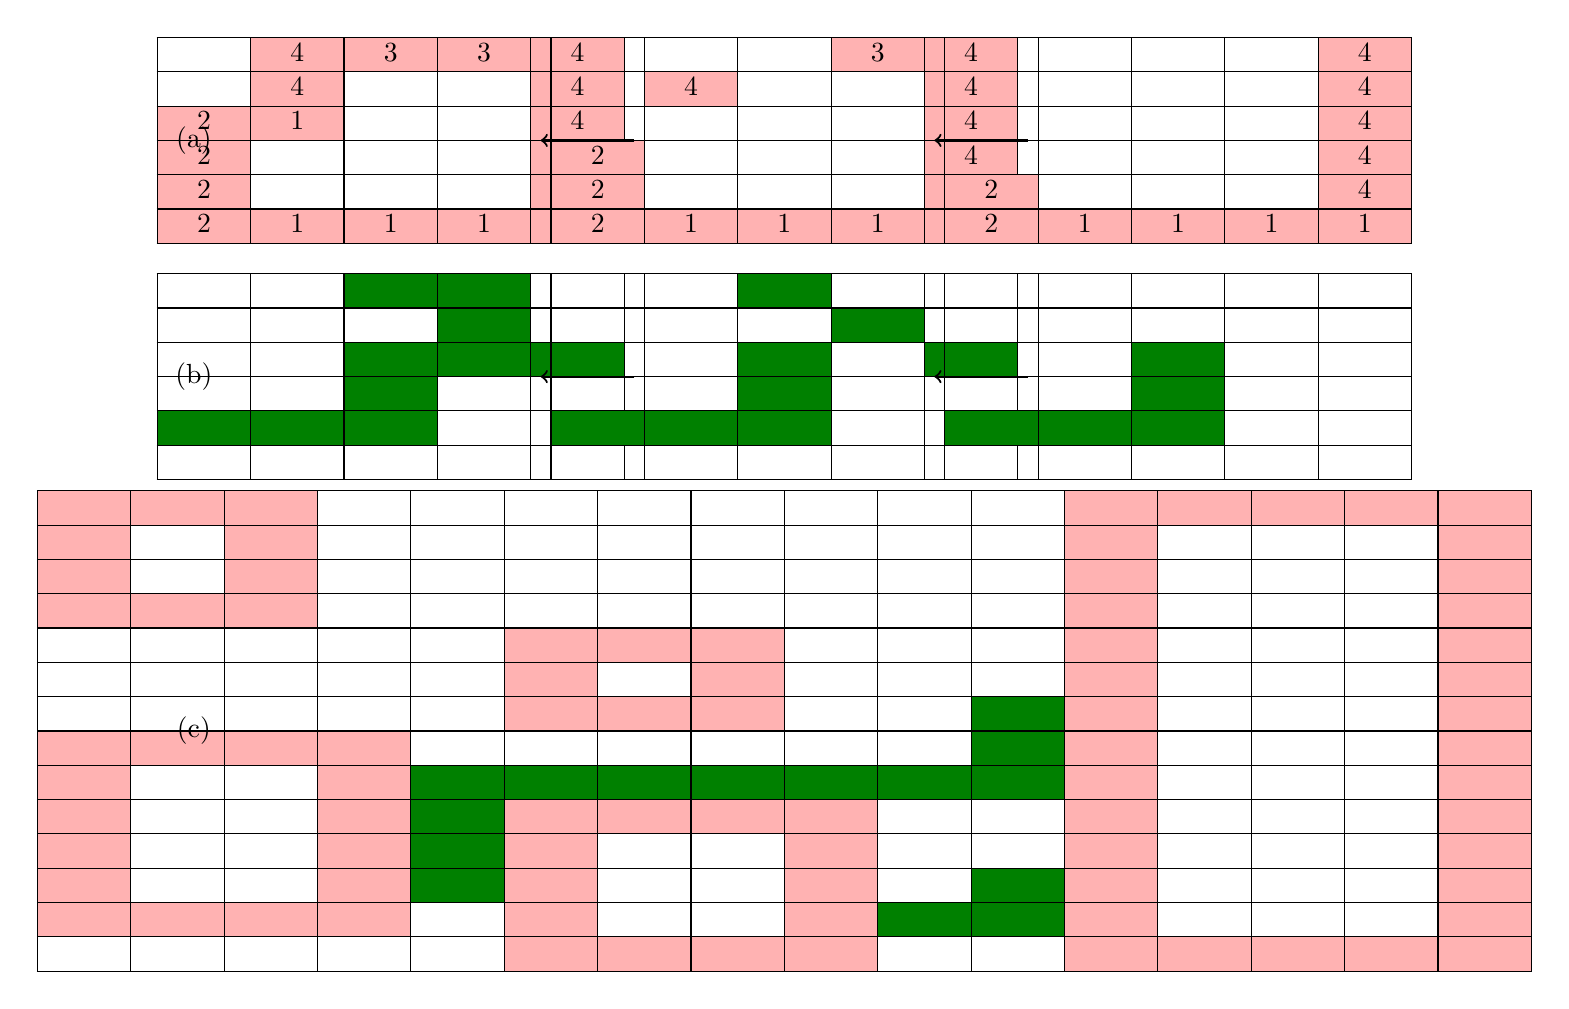
\begin{tikzpicture}

    % règle 1
    \node (tab1) at (0,0) {
        \begin{tabular}{| >{\centering\arraybackslash}m{0.75cm}
                  | >{\centering\arraybackslash}m{0.75cm}
                  | >{\centering\arraybackslash}m{0.75cm}
                  | >{\centering\arraybackslash}m{0.75cm}
                  | >{\centering\arraybackslash}m{0.75cm} |}
        \hline
         &  \cellcolor{red!30}4 &\cellcolor{red!30}3 &\cellcolor{red!30}3 &\cellcolor{red!30}4 \\
        \hline
	 & \cellcolor{red!30}4 & & &\cellcolor{red!30}4\\
        \hline
        \cellcolor{red!30}2 & \cellcolor{red!30}1  & & &\cellcolor{red!30}4\\
        \hline
        \cellcolor{red!30}2&  & & &\cellcolor{red!30}4\\
        \hline
        \cellcolor{red!30}2&  & & & \cellcolor{red!30}4\\
        \hline
        \cellcolor{red!30}2 &  \cellcolor{red!30}1 & \cellcolor{red!30}1& \cellcolor{red!30}1 & \cellcolor{red!30}1\\
        \hline
        \end{tabular}
    };

    \node (tab2) at (5, 0){
        \begin{tabular}{| >{\centering\arraybackslash}m{0.75cm}
                  | >{\centering\arraybackslash}m{0.75cm}
                  | >{\centering\arraybackslash}m{0.75cm}
                  | >{\centering\arraybackslash}m{0.75cm}
                  | >{\centering\arraybackslash}m{0.75cm} |}
        \hline
         &   & &\cellcolor{red!30}3 &\cellcolor{red!30}4 \\
        \hline
	 & \cellcolor{red!30}4 & & &\cellcolor{red!30}4\\
        \hline
         &  & & &\cellcolor{red!30}4\\
        \hline
        \cellcolor{red!30}2&  & & &\cellcolor{red!30}4\\
        \hline
        \cellcolor{red!30}2&  & & & \cellcolor{red!30}4\\
        \hline
        \cellcolor{red!30}2 &  \cellcolor{red!30}1 & \cellcolor{red!30}1& \cellcolor{red!30}1 & \cellcolor{red!30}1\\
        \hline
        \end{tabular}
    };
    \node (tab3) at (10, 0){
        \begin{tabular}{| >{\centering\arraybackslash}m{0.75cm}
                  | >{\centering\arraybackslash}m{0.75cm}
                  | >{\centering\arraybackslash}m{0.75cm}
                  | >{\centering\arraybackslash}m{0.75cm}
                  | >{\centering\arraybackslash}m{0.75cm} |}
        \hline
         &   & & &\cellcolor{red!30}4 \\
        \hline
	 &  & & &\cellcolor{red!30}4\\
        \hline
         &   & & &\cellcolor{red!30}4\\
        \hline
        &  & & &\cellcolor{red!30}4\\
        \hline
        \cellcolor{red!30}2&  & & & \cellcolor{red!30}4\\
        \hline
        \cellcolor{red!30}2 &  \cellcolor{red!30}1 & \cellcolor{red!30}1& \cellcolor{red!30}1 & \cellcolor{red!30}1\\
        \hline
        \end{tabular}
    };


    \draw[->, thick] (tab1) -- (tab2);
    \draw[->, thick] (tab2) -- (tab3);
    %\node at (1.5, 0.8) {$\delta_e(q, b) = (q', b',  -1)$};
    %\node at (1.5, 1.2) {$s \in \{\texttt{<}, \texttt{>}\}$};
    
    

    % règle 3
    \node (tab5) at (0,-3) {
         \begin{tabular}{|p{0.75cm}|p{0.75cm}|p{0.75cm}|p{0.75cm}|p{0.75cm}|}
        \hline
         &  & \cellcolor{green!50!black} & \cellcolor{green!50!black} & \\
        \hline
	 & & & \cellcolor{green!50!black} &\\
        \hline
         &  & \cellcolor{green!50!black}& \cellcolor{green!50!black} & \cellcolor{green!50!black}\\
        \hline
        &  & \cellcolor{green!50!black}& &\\
        \hline
        \cellcolor{green!50!black} & \cellcolor{green!50!black}& \cellcolor{green!50!black}& &\\
        \hline
        &  & & &\\
        \hline
        \end{tabular}    
     };

    \node (tab6) at (5,-3) {
         \begin{tabular}{|p{0.75cm}|p{0.75cm}|p{0.75cm}|p{0.75cm}|p{0.75cm}|}
        \hline
         &  & \cellcolor{green!50!black} & & \\
        \hline
	 & & & \cellcolor{green!50!black} &\\
        \hline
         &  & \cellcolor{green!50!black}& & \cellcolor{green!50!black}\\
        \hline
        &  & \cellcolor{green!50!black}& &\\
        \hline
        \cellcolor{green!50!black} & \cellcolor{green!50!black}& \cellcolor{green!50!black}& &\\
        \hline
        &  & & &\\
        \hline
        \end{tabular}       
      };
    
     \node (tab7) at (10,-3) {
         \begin{tabular}{|p{0.75cm}|p{0.75cm}|p{0.75cm}|p{0.75cm}|p{0.75cm}|}
        \hline
         &  &  & & \\
        \hline
	 & & & &\\
        \hline
         &  & \cellcolor{green!50!black}& & \\
        \hline
        &  & \cellcolor{green!50!black}& &\\
        \hline
        \cellcolor{green!50!black} & \cellcolor{green!50!black}& \cellcolor{green!50!black}& &\\
        \hline
        &  & & &\\
        \hline
        \end{tabular}           
     };

    
    \draw[->, thick] (tab5) -- (tab6);
     \draw[->, thick] (tab6) -- (tab7);
    %\node at (1.5, -1.2) {$\delta_e(q, c) = (q', c', -1)$};
    %\node at (1.5, -0.8) {$s \in \{\texttt{<}, \texttt{>}\}$};
    
    \node (tab8) at (5,-7.5) {
         \begin{tabular}{|p{0.75cm}|p{0.75cm}|p{0.75cm}|p{0.75cm}|p{0.75cm}|p{0.75cm}|p{0.75cm}|p{0.75cm}|p{0.75cm}|p{0.75cm}|p{0.75cm}|p{0.75cm}|p{0.75cm}|p{0.75cm}|p{0.75cm}|p{0.75cm}|p{0.75cm}|}
        \hline
         \cellcolor{red!30}& \cellcolor{red!30} &\cellcolor{red!30} & & & & & & & & & \cellcolor{red!30}&\cellcolor{red!30} &\cellcolor{red!30} &\cellcolor{red!30} &\cellcolor{red!30} \\
        \hline
	\cellcolor{red!30}&  & \cellcolor{red!30}& & & & & & & & &\cellcolor{red!30} & & & &\cellcolor{red!30} \\
        \hline
        \cellcolor{red!30}& & \cellcolor{red!30}& & & & & & & & &\cellcolor{red!30} & & & &\cellcolor{red!30} \\
        \hline
        \cellcolor{red!30}&\cellcolor{red!30}  &\cellcolor{red!30} & & & & & & & & &\cellcolor{red!30} & & & &\cellcolor{red!30} \\
        \hline
        &  & & & & \cellcolor{red!30}& \cellcolor{red!30} & \cellcolor{red!30}& & & &\cellcolor{red!30} & & & &\cellcolor{red!30} \\
        \hline
        &  & & & & \cellcolor{red!30}& &\cellcolor{red!30} & & & & \cellcolor{red!30}& & & &\cellcolor{red!30} \\
        \hline
        &  & & & &\cellcolor{red!30} &\cellcolor{red!30} & \cellcolor{red!30}& & & \cellcolor{green!50!black}&\cellcolor{red!30} & & & &\cellcolor{red!30} \\
        \hline
        \cellcolor{red!30}& \cellcolor{red!30} &\cellcolor{red!30} & \cellcolor{red!30}& & & & & & &\cellcolor{green!50!black} &\cellcolor{red!30} & & & &\cellcolor{red!30} \\
        \hline
        \cellcolor{red!30}&  & & \cellcolor{red!30}&\cellcolor{green!50!black} &\cellcolor{green!50!black} &\cellcolor{green!50!black} & \cellcolor{green!50!black}& \cellcolor{green!50!black}&\cellcolor{green!50!black} & \cellcolor{green!50!black} & \cellcolor{red!30}& & & & \cellcolor{red!30}\\
        \hline
        \cellcolor{red!30}&  & & \cellcolor{red!30}&\cellcolor{green!50!black} &\cellcolor{red!30} &\cellcolor{red!30} &\cellcolor{red!30} & \cellcolor{red!30}& & &\cellcolor{red!30} & & & &\cellcolor{red!30} \\
        \hline
        \cellcolor{red!30}&  & &\cellcolor{red!30} & \cellcolor{green!50!black}&\cellcolor{red!30} & & &\cellcolor{red!30} & & & \cellcolor{red!30}& & & & \cellcolor{red!30}\\
        \hline
        \cellcolor{red!30}&  & & \cellcolor{red!30}& \cellcolor{green!50!black}&\cellcolor{red!30} & & &\cellcolor{red!30} & &\cellcolor{green!50!black} & \cellcolor{red!30}& & & &\cellcolor{red!30} \\
        \hline
        \cellcolor{red!30}&\cellcolor{red!30}  &\cellcolor{red!30} &\cellcolor{red!30} & & \cellcolor{red!30}& & &\cellcolor{red!30} &\cellcolor{green!50!black} &\cellcolor{green!50!black} & \cellcolor{red!30}& & & &\cellcolor{red!30} \\
        \hline
        &  & & & & \cellcolor{red!30}&\cellcolor{red!30} & \cellcolor{red!30}& \cellcolor{red!30}& & &\cellcolor{red!30} &\cellcolor{red!30} &\cellcolor{red!30} &\cellcolor{red!30} &\cellcolor{red!30} \\
        \hline
        \end{tabular}    
     };

   
    
  	
\node at (-2.5,0) {(a)};
\node at (-2.5,-3) {(b)};
\node at (-2.5,-7.5) {(c)};
       






\end{tikzpicture}}
\end{center}
\caption{Illustration of the stabilization process. (a) Defective red regions are progressively eliminated. (b) Green regions are removed in parallel. (c) A representative configuration after the system has stabilized.}
\label{fig:redzone}
\end{figure}
